\renewcommand*{\arraystretch}{1.1}

\subsection*{BI / read / 12}
\label{sec:bi-read-12}

\noindent\begin{tabularx}{\queryCardWidth}{|>{\queryPropertyCell}p{\queryPropertyCellWidth}|X|}
	\hline
	query & BI / read / 12 \\ \hline
%
	title & Trending Posts \\ \hline
%
	pattern & \hfill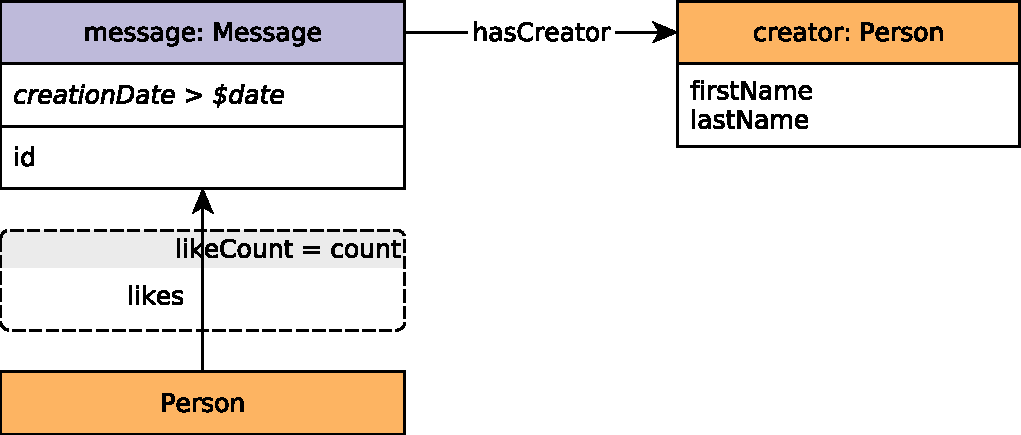
\includegraphics[scale=\patternscale,margin=0cm .2cm]{patterns/bi-read-12}\hfill\vadjust{} \\ \hline
%
	desc. & Find all Messages created after a given date, that received more than a
given number of likes.
 \\ \hline
%
	
%
	
		params &
		\innerCardVSpace{\begin{tabularx}{\attributeCardWidth}{|>{\paramNumberCell}c|>{\varNameCell}M|>{\typeCell}m{\typeWidth}|Y|} \hline
		$\mathsf{1}$ & creationDate & Date &  \\ \hline
		$\mathsf{2}$ & likeThreshold & 32-bit Integer &  \\ \hline
		\end{tabularx}}\innerCardVSpace \\ \hline
	
%
	
		result &
		\innerCardVSpace{\begin{tabularx}{\attributeCardWidth}{|>{\resultNumberCell}c|>{\varNameCell}M|>{\typeCell}m{\typeWidth}|>{\resultOriginCell}c|Y|} \hline
		$\mathsf{1}$ & message.id & 64-bit Integer & R &
				 \\ \hline
		$\mathsf{2}$ & message.creationDate & DateTime & R &
				 \\ \hline
		$\mathsf{3}$ & creator.firstName & String & R &
				The first name of the post's creator \\ \hline
		$\mathsf{4}$ & creator.lastName & String & R &
				The last name of the post's creator \\ \hline
		$\mathsf{5}$ & likeCount & 32-bit Integer & A &
				The number of Likes the Post received \\ \hline
		\end{tabularx}}\innerCardVSpace \\ \hline
	
%
	
		sort		&
		\innerCardVSpace{\begin{tabular}{|>{\sortNumberCell}c|>{\varNameCell}l|>{\directionCell}c|} \hline
		$\mathsf{1}$ & likeCount & $\desc$ \\ \hline
		$\mathsf{2}$ & message.id & $\asc$ \\ \hline
		\end{tabular}}\innerCardVSpace \\ \hline
	%
	limit & 100 \\ \hline
	%
	CPs &
	\multicolumn{1}{>{\raggedright}l|}{
		\chokePoint{1.2}, 
		\chokePoint{2.2}, 
		\chokePoint{3.1}, 
		\chokePoint{6.1}
		} \\ \hline
	%
	%
\end{tabularx}
\queryCardVSpace